\documentclass{sig-alternate}

%% Custom TeX

\usepackage{srcltx}
\usepackage{url}
%\usepackage{fullpage}
%\usepackage{fancyhdr}
\let\proof\relax
\let\endproof\relax
\usepackage{latexsym,amsthm,amsmath,amssymb,stmaryrd}

%\usepackage{charter}
%\usepackage{euler}
\renewcommand{\bfdefault}{b}

\usepackage{xspace}
\usepackage{enumerate}
%\usepackage[pdftex,hyperref,svgnames]{xcolor}
\usepackage{graphics}
%\usepackage{pstricks}
%\usepackage{color}
%\usepackage{comment}
\usepackage{listings}
\usepackage{supertabular}
\usepackage{stackrel}
\usepackage{marvosym}
\usepackage{pgf,tikz}
\usepackage{mdframed}
%\usepackage{ottlayout}
\usepackage{mathpartir}
%\usepackage{listproc}
%\usepackage{perltex}
\usepackage{etoolbox}
\usepackage{color,soul} % Highlighting

% Listings
\newcommand{\code}[1]{\text{\lstinline!#1!}}

\definecolor{lightgreen}{rgb}{.85,.95,.85}
\definecolor{lightblue}{rgb}{.85,.90,1}
\definecolor{lightred}{rgb}{.95,.85,.85}
\definecolor{lightgrey}{rgb}{.95,.95,.95}
\sethlcolor{lightred}

\definecolor{drkyellow}{rgb}{0.4,0.3,0}
\definecolor{drkred}{rgb}{0.5,0,0}
\definecolor{drkgreen}{rgb}{0,0.5,0}

\definecolor{dkgreen}{rgb}{0.1,0.40,0.1}

\definecolor{dkred}{rgb}{0.5,0,0}
\definecolor{medred}{rgb}{0.6,0,0}
\definecolor{gray}{rgb}{0.5,0.5,0.5}
\definecolor{mauve}{rgb}{0.58,0,0.82}

\newcommand{\myparagraph}[1]{\paragraph{#1.}}

\newcommand{\lstrule}{%
 \hspace{1mm}%
 \color{gray}{\rule[1.18mm]{0.8\textwidth}{0.1pt}}%
 \hspace{\fill}%
}

%% TODO: Make the listings look prettier

\lstset{ %
  language=caml,                    % the language of the code
  morecomment=[l]{--},          % add Haskell comment style
  basewidth=0.5em,
  lineskip={-2.35pt},
%  aboveskip=5mm,
%  belowskip=-5mm,
  columns=fixed,
  basicstyle=\small\ttfamily,
%  identifierstyle=\textbf,
%  keywordsprefix=\#,
  literate={->}{$\rightarrow$}2
           {=>}{$\Rightarrow$}2
           {<-}{$\leftarrow$}2
           {..}{$\cdots$}2
           {fun}{$\lambda$}1
           {||}{$\parallel$}1
           {**}{$\times$}2,
  escapechar=@,
  numbers=left,                   % where to put the line-numbers
  numberstyle=\tiny\color{gray},  % the style that is used for the line-numbers
  stepnumber=1,                   % the step between two line-numbers. If it's 1, each line 
                                  % will be numbered
  numbersep=5pt,                  % how far the line-numbers are from the code
  showspaces=false,               % show spaces adding particular underscores
  showstringspaces=false,         % underline spaces within strings
  numberblanklines=false,
  showtabs=false,                 % show tabs within strings adding particular underscores
%  frame=single,                   % adds a frame around the code
%  frame=lines,
  rulecolor=\color{gray},        % if not set, the frame-color may be changed on line-breaks within not-black text (e.g. commens (green here))
  tabsize=2,                      % sets default tabsize to 2 spaces
%  captionpos=b,                   % sets the caption-position to bottom
  breaklines=false,                % sets automatic line breaking
  breakatwhitespace=false,        % sets if automatic breaks should only happen at whitespace
  title=\lstname,                   % show the filename of files included with \lstinputlisting;
%  keywordstyle=\color{blue},          % keyword style
%  identifierstyle=\color{drkgreen},     
%  backgroundcolor=\color{lightgrey},
  commentstyle=\color{dkred}\itshape,       % comment style
  stringstyle=\color{mauve}         % string literal style
}

\lstset{emph={},emphstyle={}}%
\lstset{morekeywords={\!, (, \), \., \<, \>, ref, in, if,then,else,let, install, <,>},keywordstyle={\color{blue}\bfseries}}%

%% Theorem stuff
\theoremstyle{definition}
\newtheorem{defn}{Definition}[section]
\newtheorem{lem}{Lemma}[section]
\newtheorem{thm}{Theorem}[section]

\newcommand{\aset}[1]{\{#1\}}
\newcommand{\dom}{\mathop\textit{dom}\nolimits}

%% Names of things
\newcommand{\tvetl}{TVETL\xspace}

\newcommand{\sfmt}[1]{\textsf{#1}}
\newcommand{\sch}{\textit{ch}}
\newcommand{\loc}{\ell}
\newcommand{\sassign}[2]{#1 := #2}
\newcommand{\scase}[2]{\sfmt{case}~#1~\sfmt{of}~#2}
\newcommand{\sderef}[1]{!#1}
\newcommand{\sfalse}{\sfmt{false}}
\newcommand{\sif}[3]{\sfmt{if}~#1~\sfmt{then}~#2~\sfmt{else}~#3}
\newcommand{\sinl}{\sfmt{inl}}
\newcommand{\sinr}{\sfmt{inr}}
\newcommand{\sinstall}[2]{\sfmt{install}~#1~#2}
\newcommand{\sdeclassify}[1]{\sfmt{declassify}~#1}
\newcommand{\sref}[1]{\sfmt{ref}~#1}
\newcommand{\denot}[1]{\ensuremath{\llbracket #1 \rrbacket}}
\newcommand{\ssend}[2]{\sfmt{send}~#1~#2}
\newcommand{\strue}{\sfmt{true}}
\newcommand{\sunit}{\sfmt{unit}}
\newcommand{\sreduce}{\Downarrow}
\newcommand{\treduce}{\rightarrow}
\newcommand{\partialfun}{\rightharpoonup}
\newcommand{\ltrue}{\ensuremath{\top}}
\newcommand{\lfalse}{\ensuremath{\bot}}
\newcommand{\config}[1]{\langle{}#1\rangle{}}
\newcommand{\program}[1]{\ensuremath{\mathcal{#1}}}
\newcommand{\restr}[2]{\ensuremath{\left.#1\right|_{#2}}}
\newcommand{\modelsrcon}{\models^{r}}
\newcommand{\judge}{\vdash}
\newcommand{\xv}{p}

\newcommand{\absstate}{\Sigma^s}
\newcommand{\tvar}{x^t}

\newcommand{\traces}[1]{\mathcal{T}(#1)}
\newcommand{\tick}[1]{#1^{+}}
\newcommand{\atom}{\phi^A}

\newcommand{\tr}{t}
\newcommand{\typ}{\tau}
\newcommand{\tint}{\textit{int}}
\newcommand{\tset}{\mathcal{T}}
\newcommand{\pset}{\ensuremath{\mathcal{P}}}
\newcommand{\tnext}{\mathcal{X}}
\newcommand{\talways}{\square}
\newcommand{\tevent}{\lozenge}
\newcommand{\tuntil}{~\mathcal{U}~}
\newcommand{\tsince}{~\mathcal{S}~}
\newcommand{\tpast}{~\mathcal{P}~}
\newcommand{\tknows}[1]{\mathcal{K}_{#1}}
\newcommand{\tatmost}[1]{\mathcal{N}_{#1}}
\newcommand{\tpossible}[1]{\mathcal{L}_{#1}}
\newcommand{\tthen}{~\textit{then}~}
\newcommand{\tlast}[2]{\textit{last}(#1, #2)}
%\newcommand{\tforall}{\hbox{forall}~}
\newcommand{\texists}{\hbox{exists}~}
\newcommand{\tcurrent}[1]{\hbox{current}_{#1}~}
\newcommand{\tval}[1]{\textit{value}(#1)}
\newcommand{\trelease}{\rhd}
\newcommand{\evt}{\eta}

%% for comments
\newcommand{\comment}[3][\color{red}]{{#1{[{#2}: {#3}]}}}
\newcommand{\kris}[1]{\comment[\color{orange}]{kris}{#1}}
\newcommand{\jeff}[1]{\comment[\color{green}]{JSF}{#1}}
\newcommand{\thickhline}{\noalign{\hrule height 1pt}}
\newcommand{\low}{\text{L}\xspace}
\newcommand{\high}{\text{L}\xspace}

\newcommand{\lang}{revea$\lambda$\xspace}

%% End of custom TeX

%\conferenceinfo{XXX} {XXX}
%\CopyrightYear{XXX}
%\copyrightdata{XXX}

\begin{document}

\title{Information Flow Policies for User Interaction}
\maketitle

\begin{abstract}
  Researchers have explored a wide range of declassification policies
  in the context of \emph{batch} programs --- those that produce an
  output given an input. In this paper, we explore declassification in
  the context of \emph{interactive, GUI-based} software, such as
  mobile apps. We observe that in many apps, declassification is
  controlled by the user via the GUI, and may change over time as an
  app executes. We introduce revea$\lambda$, a core language that can
  model interactive GUI apps including user interactions, time varying
  input, and declassification. In revea$\lambda$, we use an epistemic
  temporal logic to specify security policies; the logic is powerful
  enough to capture notions of interactive declassification we have
  seen in a range of apps that deal with time varying secret input. We
  prove that many standard security and declassification properties
  have counterparts in our logic, including a set of new polices that
  cannot be expressed in prior work.  We also show how to use symbolic
  execution to check these policies, presenting a concrete
  counterexample (in the form of a user input sequence along with a
  set of secret inputs) when one exists.  We implement our symbolic
  execution semantics in a symbolic executor for Android and apply it
  to a range of example apps.
\end{abstract}

% This leads developers to adding a number of potentially unsound and
% awkward declassification measures to languages which cannot cleanly
% express declassification information.

\section{Introduction}
\label{sec:introduction}

\kris{This text is really bad.}

Decades of language based security research focuses on specifying
policies for applications, and enforcing that these policies are
respected by the program text.  As an example, one popular property is
noninterference: no private information is leaked to a public observer
(e.g., none of the user's contact information is leaked to the
internet).  However, noninterference applies to applications which run
primarily in batch mode.  By contrast, many applications built today
(such as GUIs, games, or web applications) declassify information that
the user specifies based on their interaction with the application.
Additionally, many of these applications have a notion of the
\emph{current} policy, that can be configured by the user at runtime.
For example, a user may be presented with a list of contacts, and
asked to select one, and enforce that only the selected contact is
revealed.  As many practical applications (such as password checkers)
leak some amount of information about the secret input,
declassification has been an active research area.  However, it is
still unclear how to apply it to programs.  Because of this, many
security properties that can be enforced by traditional means are
insufficient in modern interactive applications.
{
As an example, many applications running on mobile devices request access
to privilaged resources (such as the list of contacts, or fine grained
location information, or call history).  
Currently this access is granted to the whole
application, but software engineering best practices dictate that the
programmer inform the user of the app's collection of data by either
explicitly asking for permission, or putting some visible indicator
(such as an icon in the taskbar).  While the user may wish to use the
application, they may also be hesitant to believe that the application
is being faithful to best practices, and may want to verify that the
practices are respected.  A simple high level statement may be
something of the form, ``the user is always queried before access to
the contacts is granted,'' or ``whenever an application is collecting
location information, an icon is illuminated.''  These policies both
talk about a combination of several elements:

\begin{itemize}
\item The application's interaction protocol with the user
\item The time at which various events happen (the user is presented
  with a box requesting permission)
\item The set of facts that are allowed to be known when some set of
  events has happened.
\end{itemize}

In this work we develop a programming language, \lang, in which 
developers can write interactive applications 

formalism on top of temporal epistemic logic that can
express these facts, and other policies such as policies based on
configuration options, verified auditing, and more.  In this work, we
identify a class of realistic security policies for interactive
programs based on the observation that interaction with the user
interface dictates the user's \emph{intent} to declassify certain
secret information.  We furthermore identify that this
declassification happens in a controlled way dictated by the user's
interaction. \kris{also repetitive...}

Specifically, we present the following:

\begin{itemize}
\item A formlism for developing interactive applications that includes
  core GUI elements, communication with remote principals (such as
  webservices), and operations over the user's private data.

\item New time varying epstemic temporal logic

\item Proofs that previous epistemic temporal logic work can be
  ``lifted'' to our logic.

\item A set of example programs in our language, and corresponding
  formalizations in our logic, to demonstrate the completeness of our
  logic with respect to realistic policies.

\item A way to do check a subset of ETL formulas (dealing with gradual
  release) using symbolic execution.

\item Proofs that several example programs satisfy their stipulated
  security policies.
\end{itemize}

\section{Examples}
\label{sec:examples}

In the examples that follow, we follow the notation of keeping
channels prefixed with a \code{c} as to destinguish them.  \kris{I
  think for the actual paper it would be best to think of a notation
  for them, perhaps with a superscript c or something?}

\kris{Policies are not systematically defined anywhere, this needs to
  happen.}

\subsection{Sharing a designated contact}
\label{example:contacts}

Imagine an application that interacts with a remote server that allows
a user to backup selected contacts so that they may later be
retrieved.  The set of the user's contacts is private information, and
the app will query the user to pick a contact to send to the service
so that it may be backed up.  The property we wish to maintain is that
the server can never learn the value of a contact until it has been
selected from the list.

%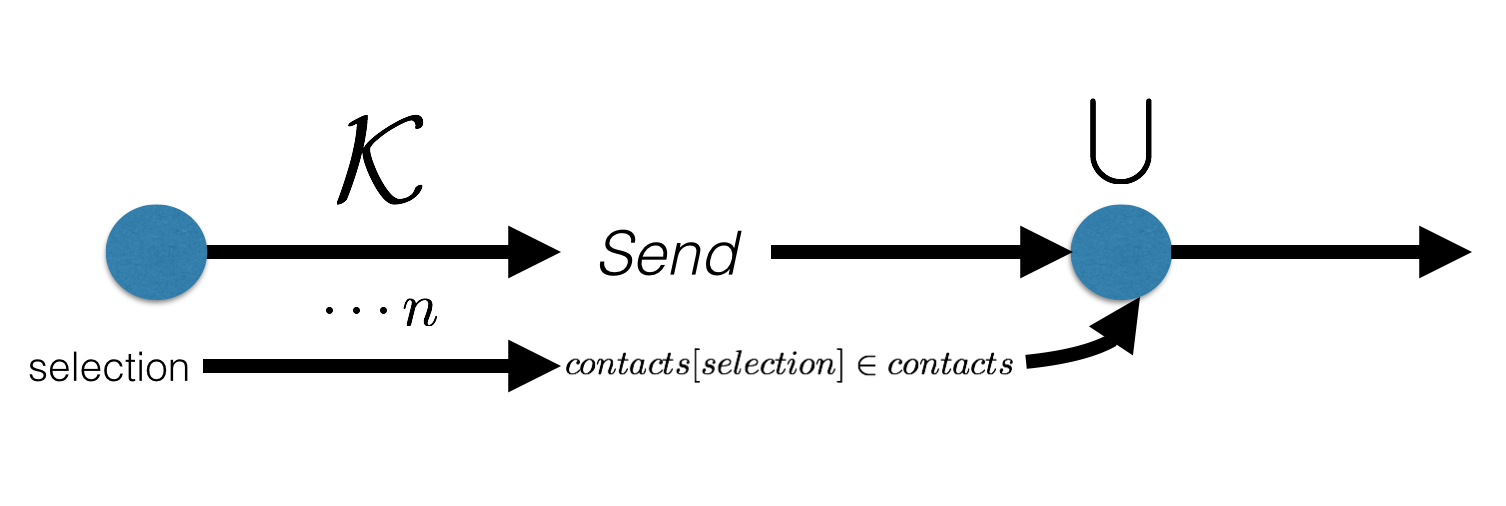
\includegraphics[width=\linewidth]{contactpickerpolicy}

\begin{lstlisting}
let cur_contact = ref None

let handle_s s =
  current_contact := Some s

let handle_b () =
  case (!cur_contact) of
    | None -> ()
    | Some s -> send net s

let onCreate (contacts) = 
  new_button id_b "Send contact";
  install id_b handle_b;
  new_spinner id_s contacts "Contacts";
  install id_s handle_s
\end{lstlisting}

In this case, the program manipulates a free variable containing a
private list of contacts, the type of which is \code{list(string)}.
The program creates a spinner whose values range over the list of
contacts, and creates a button which the user can click.  The program
then repeatedly waits for the user to either select a new contact, or
presses a button to select the current contact.  The program first
checks to ensure that some contact has been selected.

\begin{displaymath}
  \begin{array}{c}
    \code{id_b} \wedge \code{id_s} = {s}
    \trelease
    s \in contacts
  \end{array}
\end{displaymath}

\subsection{Bump app: a bunch of checkboxes}

This is an application that has a button and a certain set of
contacts.  We want to reason that whenever the attacker can infer the
phone number or email, it was proceeded by a release of the data,
which means that the email checkbox went to one, and then the button
was clicked, without any intermediary changes in the email checkbox
value (or number..).

\begin{lstlisting}
let email_release = ref false
let phone_release = ref false

let handle_b =
  if email_release && phone_release then
    send net (email ^ "|" ^ phone)
  else if email_release
    send net email
  else if phone_release
    send net phone

let handle_c r v =
  r := v
    
let onCreate (email,phone) = 
  new_checkbox id_e "Email?";
  install id_e (handle_c email_release);
  new_checkbox id_ph "Phone #?";
  install id_ph (handle_c phone_release);
  new_button id_b "Send";
  install id_b handle_b
\end{lstlisting}

The policy in this case is the following:

Whenever the button is clicked (a \code{send} event is handled), if
the email box is currently selected, then add that to the current
knowledge.  If the number box is selected, then add that to the
current knowledge.

\begin{displaymath}
  \begin{array}{c}
    \code{id_b} \wedge \code{id_e} = \strue
    \trelease \code{email} \\
%    \wedge 
    \code{id_b} \wedge \code{id_ph} = \strue
    \trelease \code{phone}
 \\
  \end{array}
\end{displaymath}  

% \begin{array}{l}
% \text{id\_send} \wedge last(\text{id\_numberBox}) = 1 ~~ Releases ~~ value(number)
% \end{array}
% \end{displaymath}

% \begin{displaymath}
% \begin{array}{l}
% \text{id\_send} \wedge last(\text{id\_emailBox}) = 1 ~~ Releases ~~ value(email)
% \end{array}
% \end{displaymath}

\subsection{Toggling resolution of collected data}

Many apps include access to time varying data sources, such as
location information.  The user may feel uncomfortable revealing their
fine grained information to the application, but may be okay revealing
their location when they allow it: e.g., when they check a box.
Because of this, the app might present a configuration option to the
user that allows them to toggle the data collection between fine
grained and coarse grained information.  As an example, a restaurant
recommendation might have options that give ads to the user based on
their city, but might also recommend restaurants in their
neighborhood.

One example implementation might use a checkbox to select whether the
app should be sharing fine grained information, and collect
information only at times when the checkbox is checked:

\begin{lstlisting}
type prec = Truncate | Full
let prec_policy = ref Truncate

let handle_r v =
  if v = 0 then
    prec_policy := Truncate
  else if v = 1 then
    prec_policy := Full

let handle_loc loc = 
  case !prec_policy of
    Truncate -> send net (declassify (truncate loc))
  | Full -> send net (declassify loc)
  
let onCreate () = 
  new_radio_buttons id_r
    [(0, "Truncate"); (1, "Full precision")];
  install id_r handle_r;
  install loc handle_loc
\end{lstlisting}

\begin{displaymath}
  \begin{array}{c}
    \code{id_r} = {0} \trelease value(\code{truncate}(loc))
    \\
    \code{id_r} = {1} \trelease value(loc)
    \\
%    [\forall x . (\code{loc}, x) \wedge (\nexists y . \tlast{\code{id_r}}{y}) \trelease
%    \code{truncate}~x]
  \end{array}
%  \begin{array}{l}
%last(\text{id\_checkbox}) = 1 ~~ Releases ~~ value(last(\text{location}))
%\end{array}
\end{displaymath}

\subsection{Geofencing app}

\kris{policy not done yet}

This is an app that responds to requests for the collected
information, as long as the user is within a certain designated area.

\begin{lstlisting}
let last_loc = ref (0, 0)

let handle_net_in () =
  if in_bounds (!last_loc) then
    send net last_loc

let handle_loc loc =
  if (can_satisfy(loc))
    last_loc := loc
  
let onCreate = 
  install loc handle_loc;
  install net_in handle_net_in
\end{lstlisting}

\begin{displaymath}
  \begin{array}{c}
    \forall x . (\code{net_in}, ()) \wedge \tlast{\code{loc}}{x}
    \wedge (\textit{in\_bounds}~x) \trelease x
  \end{array}
\end{displaymath}

\jeff{The above policy assumes we can check the \emph{in\_bounds}
  predicate and that it's the same as \code{in_bounds}. A bit yucky
  and perhaps not interesting.}

\subsection{Continuous/intermittent location app}

\kris{policy not done yet}

\begin{lstlisting}
let last_loc = ref (0, 0)

let continuous = ref false

let handle_loc loc =
  last_loc := loc;
  if (!continuous)
    send net loc

let handle_c v =
  continuous := v

let handle_b () =
  send net (!last_loc)

let onCreate =
  install loc handle_loc;
  new_checkbox id_c "Continuous map update?";
  install id_c handle_c;
  new_button id_b "Show my location";
  install id_b handle_b
\end{lstlisting}

\begin{displaymath}
  \begin{array}{c}
    [\forall x . (\code{loc}, x) \wedge \tlast{\code{id_c}}{\strue}
    \trelease x] \\
    \wedge
    [\forall x . (\code{id_b}, ()) \wedge \tlast{\code{id_c}}{\sfalse}
    \wedge \tlast{\code{loc}}{x} \trelease x] \\
    \wedge
    [\forall x . (\code{id_b}, ()) \wedge (\nexists y . \tlast{\code{id_c}}{y})
    \wedge \tlast{\code{loc}}{x} \trelease x] \\
  \end{array}
\end{displaymath}

\section{Language Formalism}
\label{sec:formalism}

In this section we present the formalism of the operational sematnics
of a programming language for a reactive semantics that allows handling
messages on a message queue.  Programs make progress by sending messages on
channels, and responding to messages sent on channels.  In this way,
programs can respond to various user input (GUI elements) and also
communicate back and forth with third parties (via channels that are
handled over the network).

\begin{figure}[t]
  \begin{displaymath}
    \begin{array}{lrcl}
      \hbox{prims} & \xv & ::= & n \mid f(\xv_1, \ldots, \xv_i)  \\
      \hbox{values} & v & ::= & \xv \mid \loc \mid \lambda x.e \\
      % \mid \sch
      \hbox{exprs} & e & ::= &
      v
      \mid x
      \mid e_1~e_2
      \mid \sref{e}
      \mid \sassign{e_1}{e_2}
      \mid \;\sderef{e} \\
      && \mid & \scase{e}{\aset{f(x_{i1}, \ldots, x_{ij}) \rightarrow
          e_i}_{i\in 1..k}} \\
      && \mid & \sinstall{\sch}{e}
      \mid \ssend{\sch}{e}
      \mid \sdeclassify{e} \\
      \hbox{constrs} & f & ::= &
      \sfmt{none} \mid \sfmt{some} \mid \sunit \mid \cdots \\
      \hbox{channels} & \sch^{\{i,o\}} & ::= & \sfmt{netin} \mid \sfmt{netout}
      \mid \cdots \\
%      \hbox{types} & \typ & ::= & \tint \mid \sch(\typ_1, \ldots, \typ_i) \\ \\
    \end{array}
  \end{displaymath}    

  % \begin{displaymath}
  %   \begin{array}{ll}
  %     \loc \in \textit{Locations}
  %   \end{array}
  % \end{displaymath}
    
  \begin{displaymath}
    \begin{array}{rcll}
      \Sigma & = & (M, \sigma, H,i) & \hbox{State} \\
      \evt & : & \sch ? p \mid \sch ! p \mid \tau & \hbox{Message} \\
      M, t & : & \evt ~ \textit{list} & \hbox{Message queue, trace}\\
      \sigma & : & \loc \partialfun  v & \hbox{Heap} \\
      H & : & \sch \partialfun \lambda x.e & \hbox{Handler map} \\
      S & : & \sch \rightarrow i \rightarrow p & \hbox{Secrets}
    \end{array}
  \end{displaymath}
  \caption{Source language syntax and semantic definitions}
  \label{fig:lang}
\end{figure}

\emph{Primitives}~$xv$ are those values that may appear in events
(e.g., button clicks, network sends) in the message queue. Primitives
consist of integers and terms built from constructors $f$, e.g.,
\sfmt{none}, \sfmt{some}, etc. In Section~\ref{sec:examples} we used
the unit value $()$, which we can encode as a nullary constructor
$\sunit$.

\emph{Values}~$v$ consist of primitives, heap locations~$\loc$, and
lambdas. \emph{Expressions}~$e$ are mostly standard, and include
values, variables~$x$, function applications~$e_1~e_2$, memory
allocation~$\sref{e}$, assignment~$\sassign{e_1}{e_2}$, and
dereference~$\sderef{e}$.  Expressions also includes the pattern
matching form \sfmt{case}, which evaluates its first argument to some
constructed term and then evaluates whichever rule matches. We omit
standard conditionals, since they can be encoded as two nullary
constructors $\strue$ and $\sfalse$ with pattern instead of the
standard $\sfmt{if}\ldots\sfmt{then}\ldots\sfmt{else}$ form.

The last three expression forms are particular to our
setting. $\sinstall{\sch}{e}$ installs $e$ (which must evaluate to a
lambda) to receive messages on a channel $\sch$; as we saw
previously, channels may include the network (\sfmt{netout},
\sfmt{netin}), channels for GUI events such as button clicks, and
channels for location updates. The network channels are distinguished
in the sense that the adversary is assumed to have access to them,
whereas all other channels are assumed to be private to the user.

The expression $\ssend{\sch}{e}$ sends $e$ (which must evaluate to a
primitive) over a channel. Finally, $\sdeclassify{e}$ marks an
expression the programmer intends to send over the network.


\begin{figure*}[t]
  \small
  \begin{displaymath}
    \begin{array}{c}
      \multicolumn{1}{l}{
        \framebox{$e, \Sigma_1 \sreduce v, \Sigma_2$}
      }
      \\ \\

      \infer[RVal]
      { }
      { v, \Sigma \sreduce v, \Sigma }

      \qquad

      \infer[RApp]
      {
        e_1, \Sigma_1 \sreduce (\lambda x.e_3), \Sigma_2 \\
        e_2, \Sigma_2 \sreduce v_1, \Sigma_3 \\\\
        \aset{x\mapsto v_1}e_3, \Sigma_3 \sreduce v_2, \Sigma_4
      }
      { e_1\;e_2, \Sigma_1 \sreduce v_2, \Sigma_4}

      \qquad

      \infer[RRef]
      {e, \Sigma_1 \sreduce v, \Sigma_2 \\
        \loc \not\in \dom(\Sigma_2.\sigma) \\\\
        \sigma' = \Sigma_2.\sigma[\loc\mapsto v]
      }
      {\sref e, \Sigma \sreduce \loc, \Sigma_2[\sigma \mapsto \sigma']}

      \qquad

      \infer[RAssign]
      {e_1, \Sigma_1 \sreduce \loc, \Sigma_2 \\
        \loc \in \dom(\Sigma_2.\sigma) \\\\
        e_2, \Sigma_2 \sreduce v, \Sigma_3 \\
        \sigma' = \Sigma_2.\sigma[\loc \mapsto v]
      }
      {\sassign {e_1} {e_2}, \Sigma_1 \sreduce
        v, \Sigma_2[\sigma \mapsto \sigma']}

      \\ \\

      \infer[RDeref]
      {e, \Sigma_1 \sreduce \loc, \Sigma_2 \\
       \Sigma_2.\sigma(\loc) = v}
      {\sderef e, \Sigma_1 \sreduce v, \Sigma_2 }

      \qquad

      \infer[RCase]
      {e_1, \Sigma_1 \sreduce f(v_1, \ldots, v_n), \Sigma_2 \\
        \aset{x_i\mapsto v_i}_{i\in 1..n}e_2, \Sigma_2 \sreduce v, \Sigma_3
      }
      {\scase{e_1}{\aset{\ldots, f(x_1, \ldots, x_n) \rightarrow
          e_2, \ldots}}, \Sigma_1 \sreduce v, \Sigma_3}
      \\ \\

      \infer[RInst]
      {
        e_1, \Sigma_1 \sreduce (\lambda x.e_2), \Sigma_2 \\
        H' = \Sigma_2.H[\sch \mapsto \lambda x.e_2]
      }
      {
        \sinstall \sch {e_1}, \Sigma_1 \sreduce \sunit, \Sigma_2[H
        \mapsto H']
      }

      \qquad

      \infer[RSend]
      { e, \Sigma_1 \sreduce \xv, \Sigma_2 \\
        M' = \Sigma_2.M, (\sch, \xv)
      }
      { \ssend \sch e, \Sigma_1 \sreduce \sunit, \Sigma_2[M \mapsto M']}

      \qquad

      \infer[RDeclassify]
      {e, \Sigma_1 \sreduce v, \Sigma_2}
      {\sdeclassify{e}, \Sigma_1 \sreduce v, \Sigma_2}

      \\ \\

      \multicolumn{1}{l}{
        \hbox{\textit{In machine state $\Sigma_1$, expression $e$ reduces to
          value $v$ and updates machine state to $\Sigma_2$.}}
      }

      \\ \\ 

      \multicolumn{1}{l}{
        \framebox{$\Sigma_1 \treduce^{\evt} \Sigma_2$ \hbox{ and } $S
          \judge e \sreduce t$}
      }
      \\ \\

      \infer[THandle]
      { \Sigma_1.M = (\sch^{\{i,s,u\}}, \xv), M' \\
        \Sigma_1.H(\sch) = \lambda x.e \\\\
        \Sigma' = \Sigma_1[M\mapsto M'] \\
        e \aset{x \mapsto \xv}, \Sigma' \sreduce v', \Sigma_2 \\
      }
      { \Sigma_1 \treduce^{\tau} \tick{\Sigma_2} }

      \qquad

      \infer[TOutput]
      { \Sigma.M = (\sch^o,p), M' \\\\
        \Sigma' = \Sigma[M\mapsto M']
      }
      { \Sigma \treduce^{\sch^o!p} \tick{\Sigma'}}
      
      \qquad

      \infer[TSecInput]
      { \Sigma' = \Sigma[M \mapsto \Sigma(M) @ (\sch^i, S_{\sch^i}(\Sigma.i))]
      }
      { \Sigma \treduce^{\sch^i?p} \tick{\Sigma'} }

      \\ \\ 

      \infer[TInput]
      { \Sigma' = \Sigma[M \mapsto \Sigma(M) @ (\sch^i , p)] \\\\
        \sch^i \in \dom(\Sigma.H)
      }
      { \Sigma \treduce^{\sch^i?p} \tick{\Sigma'} }

      \qquad

      % \infer[TLookupSecret]
      % { \Sigma.M = (\sfmt{getsecret},\sch^s,i), M' \\\\
      %   \Sigma' = \Sigma[M\mapsto M' @ (\sch, \Sigma.S(\sch)(\Sigma.i))]
      % }
      % { \Sigma \treduce^{(\sch, \Sigma.S(\sch)(\Sigma.i))} \Sigma'}
      
      % \\ \\ 

      \infer[TProg]
      {
      \Sigma_0 = ([(\code{onCreate},\code{unit})]
                  ,\emptyset
                  ,\aset{\code{onCreate} \mapsto
                          \lambda x . S(e)})
      \quad x \not\in FV(e) 
        \\\\ 
      \Sigma_i \treduce^{\evt_i} \Sigma_{i+1}
      \quad i \in [0..n]
      }
      { S \judge e { \sreduce \evt_0 \cdot \evt_1 \cdots \evt_n } }

      \\ \\
      \multicolumn{1}{l}{
        \hbox{\textit{Machine state $\Sigma_1$ steps to state $\Sigma_2$ generating
            message $\eta$, and given secret inputs $S$, program $e$
            generates \tr.}}
      }

    \end{array}
  \end{displaymath}
  \caption{Operational semantics}
  \label{fig:semantics}
\end{figure*}

\paragraph*{Semantics}

Figure~\ref{fig:semantics} gives an operational semantics for our
language. The semantics uses the definition of a \emph{state}~$\Sigma$
from Figure~\ref{fig:lang}. A machine state $(M, \sigma, H)$ include a
\emph{message queue}~$M$, a list of \emph{messages}~$\evt$, which are
channel, primitive pairs; a \emph{heap}~$\sigma$, which maps locations
to values; and a \emph{handler map}~$H$, which maps a channel name to
the function installed to handle events on that channel. We also write
$t$ for message queues that are \emph{traces} of externally visible
messages; more on this below.  To keep our semantics concise, we write
$\Sigma.X$ (where $X$ could be $M$, $\sigma$, or $H$) to mean the $X$
component of $\Sigma$. Similarly, we write $\Sigma[X\mapsto X']$ to
mean $\Sigma$ where the $X$ component has been replaced to $X'$.

The top portion of Figure~\ref{fig:semantics} defines big-step
judgments of the form $e, \Sigma_1 \sreduce v, \Sigma_2$, meaning
evaluating expression $e$ in state $\Sigma_1$ produces a value $v$ and
new state $\Sigma_2$. The first several rules are standard.
\textsc{RVal} evaluates a value to itself, without changing the
state. \textsc{RApp} evaluates $e_1$ to a lambda, evaluates $e_2$ to
a value, and then evaluates the body of the lambda with the actual
argument substituted for the formal variable.

\textsc{RRef} evaluates $e$ to a value $v$, finds a fresh location
$\loc$ in the heap, and then evaluates to $\loc$, returning a state
where the heap maps $\loc$ to $v$. \textsc{RAssign} evaluates $e_1$
to a location $\loc$ and then updates the contents of
$\loc$. \textsc{RDeref} evaluates $e$ to a location and returns the
contents of that location. \textsc{RCase} evaluates $e_1$ to a
constructed term and then evaluates the matching expression with the
pattern variables $x_i$ replaced by the corresponding values
$v_i$. This rule is non-deterministic if there is more than one
matching pattern, but by convention we assume this does not occur.

\textsc{RInst} evaluates $e_1$ to a lambda and adds it as a handler
for channel $\sch$; the result value is the unit value
$\sunit$. \textsc{RSend} evaluates $e$ to a primitive $\xv$, and then
adds the message $(\sch, \xv)$ to the end of the message
queue. Finally, \textsc{RDeclassify} simply evaluates the expression;
this form has no run-time effect in the standard semantics.
\jeff{That seems weird---is there something we need to do to the
  semantics here?}

\paragraph*{Trace Generation}
As we saw in Section~\ref{sec:examples}, programs in our language
actually execute as a series of handlers that consume inputs and
produce outputs, quiescing in between each handler until a new input
arrives. The bottom part of Figure~\ref{fig:semantics} presents rules
that orchestrate this process.

The first three rules prove judgments of the form $\Sigma_1
\treduce^{\evt} \Sigma_2$, meaning the machine in state $\Sigma_1$
produces a new state $\Sigma_2$, possibly involving an action $\evt$
visible to either the user or the adversary.

\textsc{THandle} consumes a message $(\sch, \xv)$ from the front of
the message queue (recall \textsc{RSend} adds a message to the
\emph{back} of the message queue), looks up the handler for $\sch$,
and then invokes the handler, passing $\xv$ as its argument. Notice
that the handler is invoked as a big-step; thus, handler execution is
always atomic. \jeff{Say more?}  Running a handler is not an
externally visible operation, which is indicated by an empty
message $\cdot$ on the reduction arrow.

\textsc{TOutput} models the network, consuming a single message from
\sfmt{netout}. Since the message may be seen by the adversary, it
decorates the reduction arrow. Finally, \textsc{TInput} models an
input message coming into the system, either from the user or from the
adversary (on \sfmt{netin}). The rule non-deterministically chooses
some $\sch$ for which a handler is defined (recall by convention this
excludes \sfmt{netout}) and a value $p$, and sends $\sch$ the message
$p$. \jeff{What about ranges for $p$? Seems a bit icky to get into
  that, but otherwise our examples will break...} The message
decorates the reduction arrow because it is externally visible.

The last rule in the bottom right of Figure~\ref{fig:semantics},
\textsc{TProg}, proves a judgment of the form $e \sreduce t$, meaning
running the program $e$ produces a trace $t$ of externally visible
messages. This rule runs $e$ starting from the empty state, producing
a value $v$ that is discarded and an initial state $\Sigma_0$. It them
repeatedly reduces $\Sigma_i$ to produce a new state $\Sigma_{i+1}$,
possibly generating a message $\eta_0$. Then the trace $t$ produced is
the concatenation of the $\eta_i$; here empty messages $\cdot$ are
discarded from the concatenation. Notice that the length of the trace
$n$ is non-deterministic; in general, since these are reactive
programs, they can potentially run for an any number of steps as long
as additional input arrives.

\section{Epistemic Temporal Logic}

\begin{figure*}[t]
  \begin{displaymath}
    \begin{array}{rcl}
      % \phi^\mathcal{T} & ::= & x \mid p^\mathcal{T} \mid f^\mathcal{T}
      % ( \phi^{\mathcal{T}}_1 , ... , \phi^\mathcal{T}_n ) \mid
      % \\
      \phi, \psi & ::= &
      \atom ( p_1 , ..., p_n ) @ \tvar
      \mid \neg \phi
      \mid \phi \wedge \phi
      \mid \phi \vee \phi
      \mid \phi \tuntil \phi
      \mid \phi \tsince \phi \\
      & \mid & \talways \phi
      \mid \tevent \phi
      \mid \forall x . \phi
      \mid \tknows{\sch} \phi
      \mid Now(\phi,\tvar)
    \end{array}
  \end{displaymath}

  \begin{displaymath}
    \begin{array}{rcl}
      \tset, \tr, i \models \atom ( p_1 , ..., p_n ) @ j & \iff &
      \tr[j] \models^A \atom ( p_1 , ..., p_n )  \\

      \tset, \tr, i \models \neg \phi & \iff &
      \tset, \tr, i  \not \models \phi \\

      \tset, \tr, i  \models \phi \land \psi & \iff &
      \tset, \tr, i  \models \phi \hbox{ and } \tset, \tr, i  \models \psi \\

      \tset, \tr, i  \models \phi \lor \psi & \iff &
      \tset, \tr, i  \models \phi \hbox{ or } \tset, \tr, i  \models \psi \\

%      \tset, \tr, i \models \tnext \phi & \iff &
%      \tset, \tr, (i+1) \models \phi \\

      \tset, \tr, i  \models \talways \phi & \iff &
      \forall j ~.~ j \geq i \Rightarrow (\tset, \tr, j  \models \phi) \\

      \tset, \tr, i  \models \tevent \phi & \iff &
      \exists j ~.~ j \geq i \Rightarrow (\tset, \tr, j  \models \phi) \\

      \tset, \tr, i  \models \phi \tuntil \psi & \iff &
      \exists j ~.~ j \geq i \Rightarrow ((\tset, \tr, j  \models \psi)
      \hbox{ and } \\
      & & \forall k ~.~ i \leq k < j \Rightarrow (\tset, \tr, k 
      \models \phi)) \\

      \tset, \tr, i  \models \phi \tsince \psi & \iff &
      \exists j ~.~ j \leq i \Rightarrow ((\tset, \tr, j  \models \psi)
      \hbox{ and } \\
      & & \forall k ~.~ j < k \leq i \Rightarrow (\tset, \tr, k 
      \models \phi)) \\

      \tset, \tr, i  \models \forall x . \phi & \iff &
      \hbox{for all } p, (\tset, \tr, i  \models \aset{x\mapsto p} \phi) \\

      \tset, \tr, i  \models \exists x , \phi & \iff &
      \hbox{exists } p. (\tset, \tr, i  \models \aset{x\mapsto p} \phi) \\

      \tset, \tr, i  \models \tknows{\sch} \phi & \iff &
      \forall u \in \tset ~,~
      \tr[1..i] \cong^{\sch} u[1..i] \Rightarrow \\ & & 
        \tset, u, i  \models
      \phi \\

      \tset, \tr, i  \models Now(\phi,t) & \iff &
       \tset, \tr, i \models \phi \aset{t\mapsto i} \\

    \end{array}
  \end{displaymath}
  \label{fig:etl}
  \caption{Epistemic temporal logic semantics and notation.}
\end{figure*}

\begin{figure*}[t]
  \begin{displaymath}
    \begin{array}{rcl}
      \phi, \psi & ::= &
      \atom ( p_1 , ..., p_n ) @ x^t
      \mid \neg \phi
      \mid \phi \wedge \phi
      \mid \phi \vee \phi
      \mid \phi \tuntil \phi
      \mid \phi \tsince \phi \\
      & \mid & \talways \phi
      \mid \tevent \phi
      \mid \forall x . \phi
      \mid \tknows{\sch} \phi
      \mid Now(\phi,x)
    \end{array}
  \end{displaymath}
  \label{fig:etl}
  \caption{Declassification policies}
\end{figure*}

Our epistemic logic is based on that of \cite{Balliu:11}. The logic
syntax and semantics is presented in Figure~{fig:etl}.  The logic is
parameterized by a set of atomic propositions $\atom \in P^n \to
Atoms$ with a given arity, and an atomic validity judgement $\eta
\models^A \atom (p_1 , ..., p_n)$.  The judgement $\models^A$ takes a
message and atom to a boolean.  We assume a set of base connectives
(such as $\wedge$ and $\implies$) are in $Atoms$.  An example of
$Atoms$ is (\kris{note that I have prefixed the operators to make them
  in the constructor style}):

\begin{displaymath}
  \begin{array}{rcl}
    \atom & ::= & 
    value_{ch}=(p) \mid = (p_1,p_2) \mid \geq (p_1 , p_2)
  \end{array} 
\end{displaymath}

\kris{The above looks really badly typeset as to be confusing...}

\kris{Note that we have a \emph{bunch} of derived operators, and we
  don't need all of them, we need X, U, K, not and And, I think... Add
something here...?}

\subsection{A program satisfies a formula}

Figure~\ref{fig:models-rel} gives the definition of the models
relation for a given trace and index into that trace, with respect to
a set of other traces and secret.  When we talk about a program
satisfying a trace, we mean all traces the program satisfy the trace
at time 0.  We define the function $\traces{e}$ to be the set of
traces that the program generates when quantifying over secret stores.
We then define what it means for a program $e$ to satisfy a formula
$\phi$ as follows:

\[
e \models \phi \iff \forall \tr \in \traces{e}, \traces{e}, \tr , 0 \models \phi
\]

\subsection{Lifting ETL to TVETL}

Epistemic temporal logic as presented in \cite{balliu:11} deals with
batch oriented input, where variables are presented at the
initialization of the program.  The declassification policies
expressible in this logic are analogous to gradual release (\kris{they
  mention this in their paper}) and express what is known about the
initial secret input at some time in the future.  Time varying ETL as
presented here subsumes plain ETL by a simple translation where you
take the initial input to the program and give it as input at time
zero.

\paragraph*{ETL from TVETL}

Let ETL be the logic obtained by taking TVETL and replacing all atoms
$\atom@\tvar$ with $\atom$ and changing the interpretation function
accordingly.  Because we now need to explicltly pass in the set of
secrets, assume that there's also an S to the left of the turnstile
and define a set of atoms that operate on the secrets, where you'd
normally have them operating on channels in the time varyign case.

\kris{Obviously this isn't formal enough...}


If we assume that the secret input is given to the program at time
zero, then any statement in epistemic temporal logic can be expressed
in time varying epstemic temporal logic as follows: if $\phi$ is a
formula in time varying epistemic logic, then $Now(\phi',t)$ is an
equivalent formula in TVETL, where $\phi'$ is $\phi$ where all atoms
$\atom$ are replaced with $\atom@t$:

\begin{thm}{Encoding ETL in TVETL}
  For any statement $\phi$ in ETL, assuming that the secret input is
  given at time zero to the system, $\traces{e} \models^{ETL} \phi
  \iff \traces{e} \models^{TVETL} Now(\phi',t)$.
\end{thm}

\kris{Note: The above is hazy because I haven't clearly defined
  $\models^{ETL}$.  It's the logic from tne non-time varying draft of
  the paper, where $\models^{TVETL}$ is the one from this paper.}

This theorem also applies that any tool ceritfying (for example)
noninterference in ETL does the same for the case of static input in
TVETL.

\kris{There are other ways to state this theorem, instead of giving
  the secret input at the first time step we could instead assume that
  S(ch) is the constant function that outputs the value of ch in the
  non time varying semantics.}

\paragraph*{Definitions of terms used in statements}

\kris{These statements are out of date wrt the time varyign semantics,
  but by the theorem in the previous section we can apply them equally
  well.}

\begin{defn}[Free variables / secrets]
  For any program $e$, we define the free variables of $e$ by
  induction on the term structure.  We call this $FV(e)$.  In our
  setting, the set of free variables in the program is the set of
  secret inputs to the program.
\end{defn}

\begin{defn}[Derivation of a program]
  A derivation of a program is an inhabitant of $S \judge e { \sreduce
    \evt_0 \cdot \evt_1 \cdots \evt_n }$, where $S$ is an assignment
  that assigns variables in $FV(e)$.  We call $S$ the secret input of
  the derivation.
\end{defn}

\begin{defn}[Trace of a derivation]
  We can mape a derivation of a program $d$ to a trace $\tr$, which is
  the sequence of messages in the derivation.  We define this by
  recursion on the derivation structure.  The trace of a derivation is
  $trace(d)$.
\end{defn}

\begin{defn}[Trace restriction]
  Consider any trace \tr, trace restriction, $\tr\restriction_S$ is
  the trace which contains the same sequence of messages in $\tr$, but
  containing only messages on the channels in the set $S$.  Formally
  this is $filter(\lambda x \mapsto x \in S, t)$ and can be defined similarly for
  derivations by lifting over $trace(d)$.
\end{defn}

\begin{defn}[Observer]
  An observer is a set of channels.  It is convenient to think of a
  set of channels as being observable to a party, and thus to identify
  sets of channels with a principal, or rather, to identify principals
  by sets of channels that they can observe.  We use the metavariable
  $p$ to identify a principal.
\end{defn}

\begin{defn}[Trace restriction to an observer]
  We can define trace restriction to an observer by simply filtering
  out the set of channels that the observer can see, i.e.,
  $\tr\restriction_p$.
\end{defn}

\begin{defn}[Input and Output equivalent]
  Consider any trace $\tr$.  Consider an observer who can interact
  with the program by observing messages on channels in $p$ (for
  example, \code{netout} could be such a channel).  The observer will
  see all traces which have the same sequences of messages (channel,
  value pairs) as equivalent.  We call this output equivalence.  Two
  traces $\tr_1$ and $\tr_2$ are output equivalent if and only if
  $\tr_1\restriction_p \equiv \tr_2\restriction_p$, we abbreviate this
  $\tr_1 \equiv^p \tr_2$.
\end{defn}

\subsection{Noninterference}

\paragraph*{Two-trace noninterference}

\begin{defn}[Noninterference of $e$]
  We say that $e$ is noninterfering with respect to observer $p$ if,
  
  $\forall S_1, S_2, S_1 \vdash e \Downarrow \tr_1$ and $S_2 \vdash e
  \Downarrow \tr_2$, $\tr_1 \equiv^p \tr_2$.
\end{defn}

\paragraph*{Stream based NI}

\paragraph*{ETL-based noninterference}

\begin{defn}[Noninterference of $e$ in ETL]
  For any program $e$, we define the formula in ETL $ETLNI(e)$:

  \begin{displaymath}
    \begin{array}{c}
      \forall v, \talways \big( \underbrace{L_O(x_1 = v) \wedge \ldots \wedge
        L_O(x_n = v)}_{\forall x_i \in FV(e)} \big )
    \end{array}
  \end{displaymath}

  Or equivalently...

  \begin{displaymath}
    \begin{array}{c}
      \underbrace{\big(\forall x, \talways L_O(x_1 = x)\big) \wedge \ldots \wedge
        \big(\forall x, \talways L_O(x_n = x)\big)}_{\forall x_i \in FV(e)}
    \end{array}
  \end{displaymath}
\end{defn}

\begin{thm}[Equivalence of two-trace NI and ETL NI]
  It is the case that whenever two trace NI holds for a program $e$,
  then it is the case that $derivations(e) \models ETLNI(e)$, where
  $derivations(e)$ is the set of derivations of $e$.
\end{thm}

Proof of equivalence:

\begin{itemize}
\item We have two cases:
  \begin{itemize}
  \item First case: NI -> ETLNI
  \item I need to show that for any i, the formula holds
  \item Let i be chosen arbitrarily
  \item NI gives me proofs that I have two different secrets for which
    I have observationally equivalent paths.
  \item Done because I can pick any i.
  \end{itemize}
  \begin{itemize}
  \item Second case: ETLNI -> NI
  \item I need to show that for any two secrets, I have
    observationally equivalent paths.
  \item Pick any two secrets, arbitrarily.
  \item pick any trace generated by the program with secret 1, trace 1
  \item pick any trace generated by the program with secret 2, trace 2
  \item pick an index into it named i
  \item ETLNI says that up to i it is the case that traces 1 and 2 are
    observationally equivalent.
  \end{itemize}
\end{itemize}

\subsection{``What'' policies}

\paragraph*{Multi-trace ``what'' policies}

It is common to specify what can be declassified by an equivalence
relation on initial heaps.  For example, we may wish to say that the
observer can never recover any more than $length(secret)$.  We can
specify this by using an equivalence $\equiv$ relation on the secret
inupt (NID, noninterference with declassification):

\begin{displaymath}
\begin{array}{l}
    \forall S_1 S_2, \\
    ~~ S_1 \equiv S_2
    \wedge S \vdash e \Downarrow \tr_1 
    \wedge S \vdash e \Downarrow \tr_2 \\
    ~~ ~~ \Rightarrow \tr_1 \equiv^p \tr_2
\end{array}{c}
\end{displaymath}

\paragraph*{ETL based ``what'' policies}

For our ETL formulation, we assume that the above equivalence relation
$\equiv$ is a two-arity atom and use it to specify the policy (here we
assume there is only one variable, secret, you can expand this to any
set of secrets and equivalence relation on them).

\begin{displaymath}
  ETLD = \talways \big(forall x, \equiv (secret,x) \Rightarrow L(secret=x) \big)
\end{displaymath}

\begin{thm}
  Given any equivalence relation $\equiv$, if the multi trace
  declassification property holds, then the program $e$ satisfies the
  ETL formula $ETLD$
\end{thm}

\begin{itemize}
\item We have two cases:
  \begin{itemize}
  \item First case: NID -> ETLNI
  \item I need to show that for any i, the formula holds
  \item Let i be chosen arbitrarily, I have to show formula holds up
    to i.
  \item Consider any trace the program generates, and index i into the
    trace
  \item Consider any observationally equivalent trace, we need to show
    that in at least one of these traces, it is the case that
    $\equiv(secret,x)$ holds which follows trivially.
  \end{itemize}
  \begin{itemize}
  \item Second case: ETLD -> NID
  \item I need to show that for any two secrets, if they are equal up
    to $\equiv$, then I have observationally equivalent paths.
  \item Pick any two secrets, arbitrarily.
  \item Assume that $S_1 \equiv S_2$.
  \item ETLD implies that 
  \end{itemize}
\end{itemize}

\subsection{Event based declassification policies}

\paragraph*{Trace based declassification}

Todo, I need to define this in some traditional multi trace way using
equivalence relations and knowledge bounds.

\begin{defn}[Trace based declassification of $\phi(S)$ in $e$]
\end{defn}

\paragraph*{ETL based declassificiation}

We can use ETL to write down declassification formulas by using the
LTL fragment to construct declassification conditions, parameterized
by variables which are bound to portions of the input trace, and
stipulate bounds on knowledge on the output trace.

\begin{defn}[ETL based declassification of $\phi(S)$ in $e$]
  A release policy is a statement of the form $\phi^{LTL} \rhd
  \phi^{\mathcal{T}}$.  A program $e$ satisfies a set of release
  conditions if: 
  
  \begin{displaymath}
    e \models \talways 
    \Big ( 
    \big(K(\phi_1^{\mathcal{T}}) \rightarrow   P (\phi_1^{LTL}) \big )
    \land ... \land \big( K(\phi_n^{\mathcal{T}}) \implies P
    (\phi_n^{LTL}) \big) \Big)
  \end{displaymath}
\end{defn}

\begin{thm}[Equivalence of trace based declassification and ETL based
  declassification]
\end{thm}

\section{Enforcing TVETL policies with symbolic execution}

Things that need to appear in this section:

\begin{itemize}
\item Statement: We symbolically execute a subset of ETL as it applies
  to Android programs, we show the abbreviated formalism here.

\item State what that subset is precisely, presumably it's the
  policies that are in the example section.

\item Static secrets subsume symbolic execution with time varying
  data; you are only ever being \emph{more} approximate by taking time
  varying data into account.

\item Statement of how we do symbolic execution for static secrets
  (non time varying) shown in figure \ref{fig:symbolic-semantics}

\item Statement about tricks for making symbolic execution ``really
  work.'' Single path self composition, join points, etc...

\item How time varying symbolic execution works with time varying data
  (secrets need to be tagged with knowledge bounds)

\item Theorem: Symbolic execution is sound.  Basic idea for proof: we
  could have choosen any value consistent with the PER induced by the
  policy, and assuming the SMT solver is correct we get a correct
  result as defined by semantics in previous sections.
\end{itemize}

\kris{This figure is wrong, it needs to be updated to hold the actual
  semantics that I worked out in Ott, it's just not copy-pasted there
  yet.}

\begin{figure*}[t]
  \small
  \begin{displaymath}
    \begin{array}{c}
      \multicolumn{1}{l}{
        \framebox{$e, \absstate_1 \sreduce \overline{v, \absstate_2}$}
      }
      \\ \\

      \infer[RVal]
      { }
      { v, \Sigma \sreduce v, \Sigma }

      \qquad

      \infer[RApp]
      {
        e_1, \Sigma_1 \sreduce (\lambda x.e_3), \Sigma_2 \\
        e_2, \Sigma_2 \sreduce v_1, \Sigma_3 \\\\
        \aset{x\mapsto v_1}e_3, \Sigma_3 \sreduce v_2, \Sigma_4
      }
      { e_1\;e_2, \Sigma_1 \sreduce v_2, \Sigma_4}

      \qquad

      \infer[RRef]
      {e, \Sigma_1 \sreduce v, \Sigma_2 \\
        \loc \not\in \dom(\Sigma_2.\sigma) \\\\
        \sigma' = \Sigma_2.\sigma[\loc\mapsto v]
      }
      {\sref e, \Sigma \sreduce \loc, \Sigma_2[\sigma \mapsto \sigma']}

      \qquad

      \infer[RAssign]
      {e_1, \Sigma_1 \sreduce \loc, \Sigma_2 \\
        \loc \in \dom(\Sigma_2.\sigma) \\\\
        e_2, \Sigma_2 \sreduce v, \Sigma_3 \\
        \sigma' = \Sigma_2.\sigma[\loc \mapsto v]
      }
      {\sassign {e_1} {e_2}, \Sigma_1 \sreduce
        v, \Sigma_2[\sigma \mapsto \sigma']}

      \\ \\

      \infer[RDeref]
      {e, \Sigma_1 \sreduce \loc, \Sigma_2 \\
       \Sigma_2.\sigma(\loc) = v}
      {\sderef e, \Sigma_1 \sreduce v, \Sigma_2 }

      \qquad

      \infer[RCase]
      {e_1, \Sigma_1 \sreduce f(v_1, \ldots, v_n), \Sigma_2 \\
        \aset{x_i\mapsto v_i}_{i\in 1..n}e_2, \Sigma_2 \sreduce v, \Sigma_3
      }
      {\scase{e_1}{\aset{\ldots, f(x_1, \ldots, x_n) \rightarrow
          e_2, \ldots}}, \Sigma_1 \sreduce v, \Sigma_3}
      \\ \\

      \infer[RInst]
      {
        e_1, \Sigma_1 \sreduce (\lambda x.e_2), \Sigma_2 \\
        H' = \Sigma_2.H[\sch \mapsto \lambda x.e_2]
      }
      {
        \sinstall \sch {e_1}, \Sigma_1 \sreduce \sunit, \Sigma_2[H
        \mapsto H']
      }

      \qquad

      \infer[RSend]
      { e, \Sigma_1 \sreduce \xv, \Sigma_2 \\
        M' = \Sigma_2.M, (\sch, \xv)
      }
      { \ssend \sch e, \Sigma_1 \sreduce \sunit, \Sigma_2[M \mapsto M']}

      \qquad

      \infer[RDeclassify]
      {e, \Sigma_1 \sreduce v, \Sigma_2}
      {\sdeclassify{e}, \Sigma_1 \sreduce v, \Sigma_2}

      \\ \\

      \multicolumn{1}{l}{
        \hbox{\textit{In abstract state $\absstate_1$, expression $e$
            reduces to a set of abstract values and staates value $v_{1..n}$ and $\absstate_{1..n}$.}}
      }

      \\ \\ 

      \multicolumn{1}{l}{
        \framebox{$\overline{\absstate_1} \treduce^{\evt} \overline{\absstate_2}$}
      }
      \\ \\

      \infer[THandle]
      { \Sigma_1.M = (\sch^{\{i,s,u\}}, \xv), M' \\
        \Sigma_1.H(\sch) = \lambda x.e \\\\
        \Sigma' = \Sigma_1[M\mapsto M'] \\
        e \aset{x \mapsto \xv}, \Sigma' \sreduce v', \Sigma_2 \\
      }
      { \Sigma_1 \treduce^{\tau} \Sigma_2 }

      \qquad

      \infer[TOutput]
      { \Sigma.M = (\sch^o,p), M' \\\\
        \Sigma' = \Sigma[M\mapsto M']
      }
      { \Sigma \treduce^{\sch^o!p} \Sigma'}

      \\ \\ 

      \infer[TInput]
      { \Sigma' = \Sigma[M \mapsto \Sigma(M) @ (\sch^i , p)] \\\\
        \sch^i \in \dom(\Sigma.H)
      }
      { \Sigma \treduce^{\sch^i?p} \Sigma' }

      \qquad

      % \infer[TLookupSecret]
      % { \Sigma.M = (\sfmt{getsecret},\sch^s,i), M' \\\\
      %   \Sigma' = \Sigma[M\mapsto M' @ (\sch, \Sigma.S(\sch)(\Sigma.i))]
      % }
      % { \Sigma \treduce^{(\sch, \Sigma.S(\sch)(\Sigma.i))} \Sigma'}
      
      % \\ \\ 

      \infer[TProg]
      {
      \Sigma_0 = ([(\code{onCreate},\code{unit})]
                  ,\emptyset
                  ,\aset{\code{onCreate} \mapsto
                          \lambda x . S(e)})
      \quad x \not\in FV(e) 
        \\\\ 
      \Sigma_i \treduce^{\evt_i} \Sigma_{i+1}
      \quad i \in [0..n]
      }
      { S \judge e { \sreduce \evt_0 \cdot \evt_1 \cdots \evt_n } }

      \\ \\
      \multicolumn{1}{l}{
        \hbox{\textit{Abstract state set $\overline{\absstate_1}$ steps
            to set of abstract states $\overline{\absstate_2}$}}
      }

    \end{array}
  \end{displaymath}
  \caption{Symbolic execution semantics}
  \label{fig:symbolic-semantics}
\end{figure*}

\section{Implement symbolic execution for Android}

Things that need to appear in this section:

\begin{itemize}
\item Overview of symdroid

\item Runtime for symdroid w/ ETL formulas

\item Tricks that we used to get it work

\item Example programs that we actually ran it on, presumably the
  examples from the first section of the work.
\end{itemize}

\section{Related Work}
\label{sec:related-work}

%There have been several efforts to scale up traditional batch based
%security statements (such as noninterference) to an interactive
%setting.  

Bohannon et al.~\cite{Bohannon:09}: \emph{reactive noninterference}.
Noninterference for programs that react to events (such as button clicks in a GUI), 
with the web browser as a primary motivation. 
%in a trace based setting using safety
%and liveness properties, and give several methods of proving
%correctness of programs with respect to the corresponding definitions
%using bisimulation based techniques .  

O'Neill et al.~\cite{O'Neill:06}: information flow for interactive programs that
send and receive on channels. 
Follow-up work by Clark and Hunt~\cite{Clark:09} and Rafnsson et al.~\cite{Rafnsson:12}

Garg et al.~\cite{Garg:06}: a logic for specifying security policies of distributed systems.

Chadha et al.~\cite{Lee:09}: using epistemic logic to specify secrecy policies.

Ahmad and Harper~\cite{Ahmad:13}: under submission, an epistemic logic formalization of 
noninterference, including an extension to declassification.

Sabelfeld and Myers~\cite{Sabelfeld:04}: \emph{delimited release} (* MRC: which iirc eventually led to robustness *), which says the attacker can't exploit declassification to learn more information than is intended.

Li and Zdancewic~\cite{Li:05}: \emph{relaxed noninterference}, which essentially allows declassification through function application.

Sabelfeld and Sands~\cite{Sabelfeld:05}: the original survey paper on declassification.  

Balliu et al.~\cite{Balliu:11}: expressing noninterference and declassification in epistemic temporal logic.  Balliu~\cite{Balliu:13} extends to possibilistic security.

Halpern and O'Neill~\cite{Halpern:08}: semantic characterizations of secrecy with epistemic temporal logic.

Enck et al.~\cite{Enck:10}: TaintDroid, run-time taint tracking for Android.

Chong et al.~\cite{Chong:07}: SIF, information-flow analysis and program splitting for web applications, including the web-page GUI in the browser.

Jia et al.~\cite{Jia:13}: run-time enforcement of information flow policies on Android, backed by a process calculus theory.

Nanevski et al.~\cite{Nanevski:13}: \emph{Relational Hoare Type Theory}, expressing information-flow policies with dependent types.

Aucher et al.~\cite{Aucher:11}:  knowledge-based privacy policies that can change over time.

Dimitrova et al.~\cite{Dimitrova:12}: information-flow policies along with LTL, for specifying when information must be kept secret and when it may be released.

Askarov and Chong~\cite{Askarov:12}: characterizes leakage of secret information as change in attacker knowledge.

Chong and Myers~\cite{Chong:04}: declassification policies in a security-typed language.

Roesner et al.~\cite{Roesner:12}: \emph{access control gadgets}, which are UI elements that are used to effect access control policies.  Implemented in Android.

Stateful Declassification Policies for Event-Driven
Programs. Proceedings of the 27th Computer Security Foundations
Symposium (CSF 2014), Vienna, Austria, 19-22 July 2014. \kris{Cite
  this}

\section{Future Work}
\label{sec:future}

\begin{itemize}
  \item Investigate connection between TVETL and Michael / Piotrs work
    on learning values of streams over times
  \item Investigate strategies in inputs ala Rafnsson and how they can
    be encoded in ETL (we deal with synchronous input case here, where
    their semantics can ``get stuck'' with values of bottom)
\end{itemize}

\section{Conclusion}
\label{sec:conclusion}

\bibliographystyle{IEEEtran}
\bibliography{paper}

\appendix 

\end{document}

